This section provides the reader with an overview of the laser harp. The primary operational aspects of the product, from the perspective of end users, maintainers, and administrators, are defined here. The key features and functions found in the product, as well as critical user interactions and user interfaces, are described in detail. The purpose is to give the document reader/reviewer enough information about the product to allow them to easily follow the specification of requirements found in the remainder of the document.

\subsection{Features \& Functions}
The laser harp is a musical instrument that uses laser beams to simulate the strings of a traditional harp. When a user interrupts a laser beam, the system detects the interruption and plays a corresponding musical note. The primary components of the laser harp include the laser emitters, phototransistors, a Raspberry Pi for processing, and speakers for audio output. The device is designed to be user-friendly and portable.

The key features and functions of the laser harp are as follows:
Real-time Sound Playback: Produces sound immediately when a laser string is interrupted.
Multi-note Capability: Allows for simultaneous interruption of multiple laser strings to create chords.
User Interface: Provides an interface for calibration, volume control, and sound profile selection.
Portability: Designed to be lightweight and easy to transport.
Safety: Uses Class 1 lasers to ensure user safety.

\begin{figure}[h!]
	\centering
   	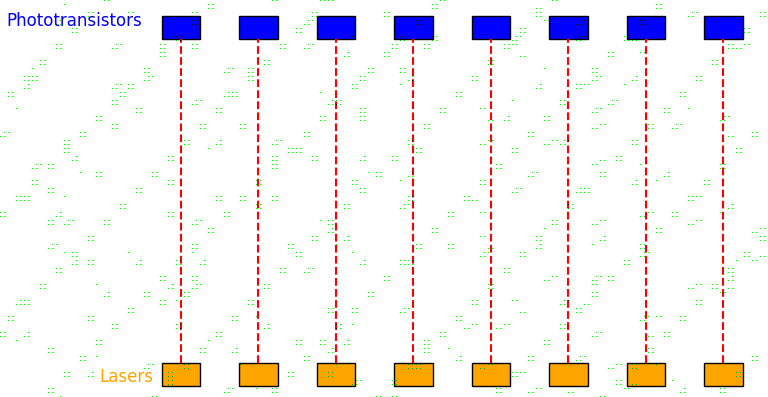
\includegraphics[width=0.60\textwidth]{images/Design}
    \caption{Laser Harp conceptual drawing}
\end{figure}

\subsection{External Inputs \& Outputs}
The laser harp interacts with external inputs and outputs as described below. The table specifies the critical data flows in and out of the system.

\begin{table}[H]
\centering
\begin{tabular}{|c|c|c|}
\hline
\textbf{Name} & \textbf{Description} & \textbf{Use} \\ \hline
Laser Interruption & Signal when a laser beam is interrupted & Detects user interaction to produce sound \\ \hline
User Input & Commands from the UI & Configures the system settings \\ \hline
Audio Output & Sound signals sent to the speakers & Produces musical notes \\ \hline
Power Supply & Electrical power input & Powers the system components \\ \hline
\end{tabular}
\caption{External Inputs and Outputs}
\end{table}

\subsection{Product Interfaces}
The laser harp includes several interfaces for user interaction, maintenance, and administration. These interfaces are designed to be intuitive and user-friendly. Below are descriptions and conceptual graphics of the key interfaces.

\textbf{User Interface:}
Calibration Screen: Allows users to calibrate the laser strings to ensure accurate detection.
Volume Control: Provides a slider to adjust the audio output volume.
Sound Profile Selection: Enables users to choose from different sound profiles for the harp.

\textbf{Maintenance Interface:}
Diagnostics Screen: Displays system status and error messages to assist in troubleshooting.
Firmware Update: Allows for updating the system software to the latest version.

\begin{figure}[h!]
	\centering
   	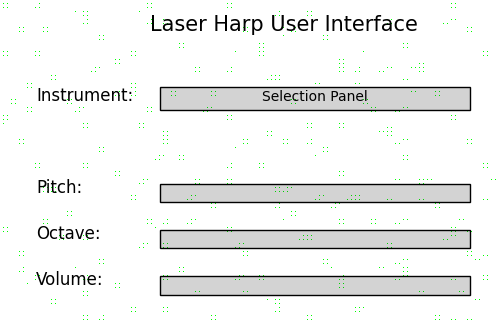
\includegraphics[width=0.60\textwidth]{images/UI}
    \caption{User Interface Mockup}
\end{figure}

The product interfaces are designed to ensure ease of use and accessibility for all users, including those with varying levels of technical expertise. These interfaces facilitate smooth operation and maintenance of the laser harp, ensuring a high-quality user experience.
